\documentclass[10pt]{article}
\usepackage[a4paper,margin=18mm]{geometry}
\usepackage{amsmath,amssymb,booktabs,array,enumitem}
\usepackage[T1]{fontenc}\usepackage{lmodern}
\usepackage{tikz}\usetikzlibrary{shapes.gates.logic.US,positioning,arrows.meta}
\usepackage[hidelinks]{hyperref}
\setlength{\parindent}{0pt}\setlength{\parskip}{4pt}
\setlength{\emergencystretch}{2em}
\newcommand{\VDD}{V_{DD}}
\newcommand{\mos}[4]{\begin{scope}[shift={(#1,#2)}]
\draw (0,.24)--(0,-.24);\draw (0,.20)--(.25,.20)--(.25,.5);
\draw (0,-.20)--(.25,-.20)--(.25,-.5);\draw (-.16,.23)--(-.16,-.23);
\ifnum#4=1\draw (-.26,0) circle (.06);\draw (-.75,0)--(-.32,0);\else\draw (-.75,0)--(-.16,0);\fi
\node[anchor=east,font=\scriptsize] at (-.76,0) {$#3$};\end{scope}}
\newcommand{\ground}[2]{\draw (#1,#2)--(#1,{#2-.12});\draw ({#1-.17},{#2-.12})--({#1+.17},{#2-.12});\draw ({#1-.11},{#2-.20})--({#1+.11},{#2-.20});}
\newcommand{\rail}[3]{\draw (#1,#2)--(#1,{#2+.14});\node[above,font=\scriptsize] at (#1,{#2+.14}) {$#3$};}
\begin{document}
\begin{center}{\Large\bfseries 2024 Midterm: corrected worked answers}\par EE3032 Introduction to VLSI, National Central University\end{center}
The two photographed prompt pages and all four supplied handwritten-answer pages were read before this report. The source sheet is graded 100, but its grade is not treated as a correctness certificate. Correct reasoning and diagrams are retained. The main numerical correction is Q6's gate-capacitance unit; Q3 also needs an explicit assumption about NAND input capacitance. All computations here use the prompt's ideal models, rather than an invented process simulation.

\section*{1. Brief answers (30 points)}
\begin{enumerate}[label=(\alph*),leftmargin=7mm,itemsep=6pt]
\item \textbf{Why not simply increase $V_{DD}$?} Supply voltage is limited by the technology's rated operating and reliability limits: stronger oxide electric field can cause breakdown and accelerate wear, and higher voltage increases switching energy roughly as $C V_{DD}^2$. Raising voltage is therefore not a free speed improvement. Retain the student's $E_{ox}\simeq V/t_{ox}$ reliability argument and add the power cost.
\item \textbf{Mask-pattern transfer.} Clean/prepare the surface; coat and bake photoresist; align the mask and expose; develop the resist; transfer the pattern to the underlying film or silicon by etching; strip the resist. If the patterned opening is for implantation, the patterned resist instead serves as its mask. The student's coat/expose/etch sequence is useful, but needs development and resist removal.
\item \textbf{FinFET sizing.} Increase or decrease the number of parallel fins (and permitted fingers/multiplicity). At fixed technology fin geometry, a tri-gate device has approximately $W_{eff}=N_{fin}(2H_{fin}+T_{fin})$; width is quantized. Retain the student's fin-count choice rather than freely changing a planar width. Fin geometry and permitted lengths are technology constrained. See the Synopsys reference below.
\item \textbf{Two static-CMOS features.} It is non-ratioed for Boolean correctness, and provides full rail-to-rail restored output levels. Device ratios still affect delay and noise margins. Retain both listed features.
\item \textbf{Two static-current mechanisms.} Subthreshold source--drain leakage in nominally off devices, and reverse-biased source/drain--body junction leakage. These are the two requested course mechanisms. Gate leakage can additionally matter in some technologies, but does not replace the requested pair.
\item \textbf{Chip-on-wafer on a silicon interposer.} Prepare the interposer wafer with TSVs and redistribution/interconnect layers; provide matching fine-pitch die/interposer bump structures; prepare and singulate the known-good dies; align and bond each die face down to the interposer wafer; underfill/protect and test the assembly. Backside thinning/TSV reveal and backside contacts complete the interposer's external connection, with detailed ordering depending on the process. The later wafer-on-substrate assembly is a separate CoWoS step. The student's TSV, microbump and face-to-face assembly ideas are retained; no unsupported proprietary fixed sequence is claimed.
\item \textbf{Backside power delivery.} Route supply/ground distribution on the wafer backside and connect it to the device power terminals using backside vias/contacts. Two advantages are reduced supply voltage drop from a less congested power path, and more frontside routing capacity for signals. Retain the student's separation of power and signal routing. Intel's PowerVia reference supports these benefits.
\item \textbf{Body effect near the output.} In a conducting stacked pull-down, bulk is tied to VSS but the source of the upper transistor can rise above VSS, so $V_{SB}$ and $V_T$ increase. The output-side device can have the largest source--body reverse bias. A stacked pMOS pull-up has the analogous well/source effect. The explanation depends on internal source voltage and body connection, not merely on naming a device's saturation region. The statement applies to the usual biased stack; it is not a universal ranking at every transient instant.
\item \textbf{Speed parameters.} From $t\sim C_L\Delta V/I_{drive}$, the principal circuit parameters are load capacitance, required voltage swing/supply, and available drive current. Current itself depends on $W/L$, mobility, oxide capacitance and overdrive/threshold. Retain the student's charge/current argument.
\item \textbf{Output capacitance.} Sum the connected downstream gate input capacitances, output-node source/drain diffusion capacitances, and routing/interconnect capacitance: $C_L=C_{gate}+C_{diff}+C_{wire}$. Retain the student's three components.
\end{enumerate}
\newpage\section*{2. MUX realization and unbuffered delay (15 points)}
\subsection*{(a) Correct 16-to-1 assignment}
\[
 f(s,x,y,z)=s\,y(x+z)+\bar s\,(x+y+z).
\]
Retain the student's select order: leaf-to-root $z,x,y,s$. Each cell chooses its left input at select 1 and its right input at select 0. The sixteen data constants from left to right are
\[1,1,1,0,0,0,0,0,\quad1,1,1,1,1,1,1,0.\]
The first eight implement $y(x+z)$ at $s=1$; the last eight implement $x+y+z$ at $s=0$. The tree has fifteen 2-to-1 cells and four stages. All sixteen assignments are independently checked by the published executable; the supplied leaf constants are correct.
\begin{center}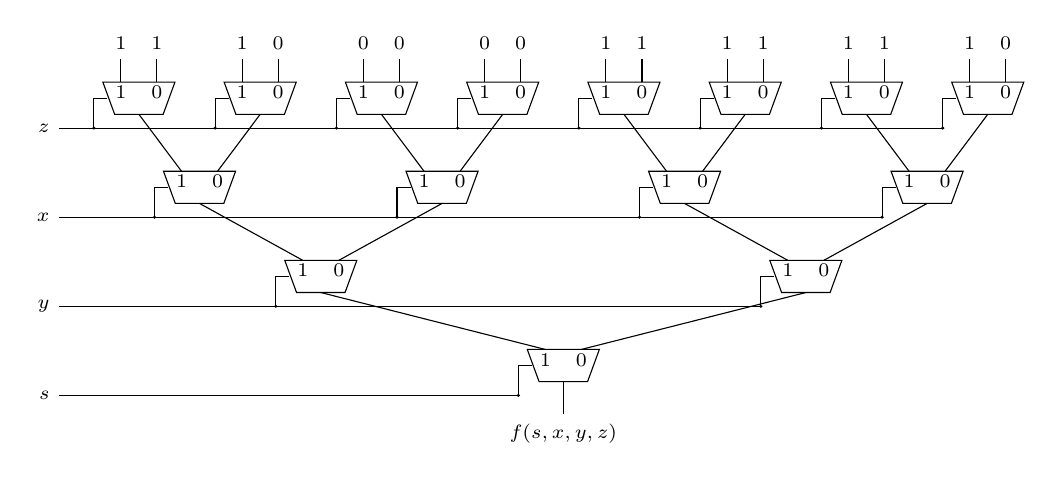
\begin{tikzpicture}[x=.88cm,y=.73cm,font=\scriptsize]
\draw (-0.520,3.280)--(0.520,3.280)--(0.350,2.720)--(-0.350,2.720)--cycle;
\node at (-0.260,3.100) {1};\node at (0.260,3.100) {0};
\draw (-0.260,3.280)--(-0.260,3.680);
\node[above] at (-0.260,3.680) {1};
\draw (0.260,3.280)--(0.260,3.680);
\node[above] at (0.260,3.680) {1};
\draw (1.230,3.280)--(2.270,3.280)--(2.100,2.720)--(1.400,2.720)--cycle;
\node at (1.490,3.100) {1};\node at (2.010,3.100) {0};
\draw (1.490,3.280)--(1.490,3.680);
\node[above] at (1.490,3.680) {1};
\draw (2.010,3.280)--(2.010,3.680);
\node[above] at (2.010,3.680) {0};
\draw (2.980,3.280)--(4.020,3.280)--(3.850,2.720)--(3.150,2.720)--cycle;
\node at (3.240,3.100) {1};\node at (3.760,3.100) {0};
\draw (3.240,3.280)--(3.240,3.680);
\node[above] at (3.240,3.680) {0};
\draw (3.760,3.280)--(3.760,3.680);
\node[above] at (3.760,3.680) {0};
\draw (4.730,3.280)--(5.770,3.280)--(5.600,2.720)--(4.900,2.720)--cycle;
\node at (4.990,3.100) {1};\node at (5.510,3.100) {0};
\draw (4.990,3.280)--(4.990,3.680);
\node[above] at (4.990,3.680) {0};
\draw (5.510,3.280)--(5.510,3.680);
\node[above] at (5.510,3.680) {0};
\draw (6.480,3.280)--(7.520,3.280)--(7.350,2.720)--(6.650,2.720)--cycle;
\node at (6.740,3.100) {1};\node at (7.260,3.100) {0};
\draw (6.740,3.280)--(6.740,3.680);
\node[above] at (6.740,3.680) {1};
\draw (7.260,3.280)--(7.260,3.680);
\node[above] at (7.260,3.680) {1};
\draw (8.230,3.280)--(9.270,3.280)--(9.100,2.720)--(8.400,2.720)--cycle;
\node at (8.490,3.100) {1};\node at (9.010,3.100) {0};
\draw (8.490,3.280)--(8.490,3.680);
\node[above] at (8.490,3.680) {1};
\draw (9.010,3.280)--(9.010,3.680);
\node[above] at (9.010,3.680) {1};
\draw (9.980,3.280)--(11.020,3.280)--(10.850,2.720)--(10.150,2.720)--cycle;
\node at (10.240,3.100) {1};\node at (10.760,3.100) {0};
\draw (10.240,3.280)--(10.240,3.680);
\node[above] at (10.240,3.680) {1};
\draw (10.760,3.280)--(10.760,3.680);
\node[above] at (10.760,3.680) {1};
\draw (11.730,3.280)--(12.770,3.280)--(12.600,2.720)--(11.900,2.720)--cycle;
\node at (11.990,3.100) {1};\node at (12.510,3.100) {0};
\draw (11.990,3.280)--(11.990,3.680);
\node[above] at (11.990,3.680) {1};
\draw (12.510,3.280)--(12.510,3.680);
\node[above] at (12.510,3.680) {0};
\draw (-1.15,2.480)--(11.600,2.480);\node[left] at (-1.15,2.480) {$z$};
\draw (-0.650,2.480)--(-0.650,3.0)--(-0.455,3.0);\fill (-0.650,2.480) circle (.027);
\draw (1.100,2.480)--(1.100,3.0)--(1.295,3.0);\fill (1.100,2.480) circle (.027);
\draw (2.850,2.480)--(2.850,3.0)--(3.045,3.0);\fill (2.850,2.480) circle (.027);
\draw (4.600,2.480)--(4.600,3.0)--(4.795,3.0);\fill (4.600,2.480) circle (.027);
\draw (6.350,2.480)--(6.350,3.0)--(6.545,3.0);\fill (6.350,2.480) circle (.027);
\draw (8.100,2.480)--(8.100,3.0)--(8.295,3.0);\fill (8.100,2.480) circle (.027);
\draw (9.850,2.480)--(9.850,3.0)--(10.045,3.0);\fill (9.850,2.480) circle (.027);
\draw (11.600,2.480)--(11.600,3.0)--(11.795,3.0);\fill (11.600,2.480) circle (.027);
\draw (0.355,1.730)--(1.395,1.730)--(1.225,1.170)--(0.525,1.170)--cycle;
\node at (0.615,1.550) {1};\node at (1.135,1.550) {0};
\draw (0.000,2.720)--(0.615,1.730);
\draw (1.750,2.720)--(1.135,1.730);
\draw (3.855,1.730)--(4.895,1.730)--(4.725,1.170)--(4.025,1.170)--cycle;
\node at (4.115,1.550) {1};\node at (4.635,1.550) {0};
\draw (3.500,2.720)--(4.115,1.730);
\draw (5.250,2.720)--(4.635,1.730);
\draw (7.355,1.730)--(8.395,1.730)--(8.225,1.170)--(7.525,1.170)--cycle;
\node at (7.615,1.550) {1};\node at (8.135,1.550) {0};
\draw (7.000,2.720)--(7.615,1.730);
\draw (8.750,2.720)--(8.135,1.730);
\draw (10.855,1.730)--(11.895,1.730)--(11.725,1.170)--(11.025,1.170)--cycle;
\node at (11.115,1.550) {1};\node at (11.635,1.550) {0};
\draw (10.500,2.720)--(11.115,1.730);
\draw (12.250,2.720)--(11.635,1.730);
\draw (-1.15,0.930)--(10.725,0.930);\node[left] at (-1.15,0.930) {$x$};
\draw (0.225,0.930)--(0.225,1.45)--(0.420,1.45);\fill (0.225,0.930) circle (.027);
\draw (3.725,0.930)--(3.725,1.45)--(3.920,1.45);\fill (3.725,0.930) circle (.027);
\draw (7.225,0.930)--(7.225,1.45)--(7.420,1.45);\fill (7.225,0.930) circle (.027);
\draw (10.725,0.930)--(10.725,1.45)--(10.920,1.45);\fill (10.725,0.930) circle (.027);
\draw (2.105,0.180)--(3.145,0.180)--(2.975,-0.380)--(2.275,-0.380)--cycle;
\node at (2.365,-0.000) {1};\node at (2.885,-0.000) {0};
\draw (0.875,1.170)--(2.365,0.180);
\draw (4.375,1.170)--(2.885,0.180);
\draw (9.105,0.180)--(10.145,0.180)--(9.975,-0.380)--(9.275,-0.380)--cycle;
\node at (9.365,-0.000) {1};\node at (9.885,-0.000) {0};
\draw (7.875,1.170)--(9.365,0.180);
\draw (11.375,1.170)--(9.885,0.180);
\draw (-1.15,-0.620)--(8.975,-0.620);\node[left] at (-1.15,-0.620) {$y$};
\draw (1.975,-0.620)--(1.975,-0.10000000000000009)--(2.170,-0.10000000000000009);\fill (1.975,-0.620) circle (.027);
\draw (8.975,-0.620)--(8.975,-0.10000000000000009)--(9.170,-0.10000000000000009);\fill (8.975,-0.620) circle (.027);
\draw (5.605,-1.370)--(6.645,-1.370)--(6.475,-1.930)--(5.775,-1.930)--cycle;
\node at (5.865,-1.550) {1};\node at (6.385,-1.550) {0};
\draw (2.625,-0.380)--(5.865,-1.370);
\draw (9.625,-0.380)--(6.385,-1.370);
\draw (-1.15,-2.170)--(5.475,-2.170);\node[left] at (-1.15,-2.170) {$s$};
\draw (5.475,-2.170)--(5.475,-1.6500000000000004)--(5.670,-1.6500000000000004);\fill (5.475,-2.170) circle (.027);
\draw (6.125,-1.9300000000000004)--(6.125,-2.5000000000000004) node[below] {$f(s,x,y,z)$};
\end{tikzpicture}\end{center}
\subsection*{(b) Delay without inserted buffers}
The selected path consists of $n$ series transmission-gate resistances. Nodes retain diffusion/wiring/load capacitance, so a signal must charge the downstream ladder through upstream resistance. Under an explicitly illustrative uniform ladder with each selected TG resistance $R$ and each of its $n$ output nodes capacitance $C$, its Elmore first moment is
\[
\tau_E=\sum_{i=1}^n R\sum_{j=i}^n C=RC\frac{n(n+1)}2=\Theta(n^2).
\]
For the four-stage path this model gives $10RC$. This is a first moment, not an exact 50\% or 10--90\% crossing time. Real coefficients depend on the node capacitances and nonlinear TG resistance; the quadratic scaling is the requested conclusion. The student correctly identifies a distributed RC ladder and quadratic stage dependence. In the ideal case of only a fixed final capacitor and zero internal capacitance, the delay instead scales as $nRC_L$; that is a different assumption.

\newpage\section*{3. Minimum-delay buffer chain (10 points)}
\textbf{Preserve polarity.} A already inverts $x$, so the dashed inserted chain must be noninverting. Add an even number of inverters: the total number $N$ of driving stages, including A, is odd.

The specified rise-time convention is $t_r=R_{p,D}C=0.05RC$, so each NAND pMOS has resistance $R/20$ and width $20W/L$ for the worst single-on-pMOS rise. This alone does not specify the NAND nMOS widths or total per-input capacitance. Q3 defines $C_g$ as the \emph{entire input capacitance of the minimum inverter}, comprising its two $W/L$ devices. If a NAND nMOS is $w_nW/L$, then
\[
C_D=\frac{20+w_n}{2}C_g,\qquad H=\frac{C_D}{C_g}.
\]
This missing width is why $C_D=20C_g$ cannot be uniquely inferred from the printed assumptions.

For equal-strength nMOS/pMOS inverter stages of size $a_i$ relative to A, $a_0=1$, and negligible parasitics,
\[
T=RC_g\left(\frac{a_1}{a_0}+\frac{a_2}{a_1}+\cdots+\frac{H}{a_{N-1}}\right).
\]
For fixed $N$, equal fanout minimizes the sum: $h=H^{1/N}$, $a_i=h^i$, and $T_N=N H^{1/N}RC_g$. The continuous optimum is $N=\ln H$, with stage effort $e$; compare the allowed odd integers rather than inserting an arbitrary parity.

\begin{center}\begin{tabular}{lrrrr}\toprule Explicit NAND assumption&$H$&$T_1/(RC_g)$&$T_3/(RC_g)$&$T_5/(RC_g)$\\\midrule
Equal NAND widths $w_n=20$&20&20&8.1433&9.1028\\
Balanced 2-series nMOS $w_n=40$&30&30&9.3217&9.8718\\\bottomrule\end{tabular}\end{center}
Both conventions select $N=3$: A plus two inserted inverters. Under the \textbf{student's intended $H=20$ assumption}, exact inserted widths for both nMOS and pMOS are $20^{1/3}W/L=2.7144W/L$ and $20^{2/3}W/L=7.3681W/L$. Using the supplied approximations gives the student's $eW/L$, $e^2W/L$ and $T\simeq3eRC_g$; retain this as an approximate conditional answer. For $H=30$, the corresponding widths are $3.1072W/L$ and $9.6549W/L$.

There are three inverter stages on the path, but only two \emph{inserted} inverters. This $T$ ends at the input of NAND D, as drawn; D's additional output delay is fixed and does not alter the optimum under the same convention.

\section*{4. Feedback NMOS gate (10 points)}
Before switching, $V_{out}=1.2$ V turns on feedback device N2. In the stated constant-on-resistance approximation, after N1 turns on the internal source node $u$ is
\[
u=1.2\frac{R}{R+2R}=0.4\ \mathrm V.
\]
N3 starts conducting when $V_{in}-u=V_{Tn}=0.4$ V; therefore the input at $x$ is $\boxed{V_{in}(t_2)=0.8\ \mathrm V}$. As output falls, N2's gate voltage falls, reducing its feedback pull-up and allowing the internal node to drop. This positive feedback assists the transition.

For the open interval $t_1<t<t_2$, $0.4<V_{in}<0.8$ V and $u\simeq0.4$ V:
\begin{center}\begin{tabular}{lll}\toprule Device&Bias check&Region\\\midrule
N1&$V_{DS}=0.4\ge V_{GS}-V_T=V_{in}-0.4$&saturation\\
N2&$V_G=V_D=1.2$, $V_S=0.4$; $V_{DS}=0.8>0.4$&saturation\\
N3&$V_{GS}=V_{in}-0.4<0.4$&cutoff\\\bottomrule\end{tabular}\end{center}
At $t_1$ N1 is just at its threshold; at $t_2$ N3 reaches its threshold and N1 reaches its saturation/linear boundary in this approximation. Do not call N3 already conducting before $t_2$, or indefinitely cutoff after output falls. Retain the student's 0.8 V and interior-interval classification with these endpoint qualifications. The voltage divider uses the supplied effective-resistance model; it is not an exact MOS square-law DC solution with body effect.

\newpage\section*{5. Noise-margin comparison (10 points)}
Every listed word makes $q=G1=\overline{BC}=1$ and $D=1$:
\begin{center}\begin{tabular}{ccccc}\toprule $ABCD$&$q$&$A$&G2 output& G3 output\\\midrule
0011&1&0&0&0\\0101&1&0&0&0\\1101&1&1&0&0\\1001&1&1&0&0\\\bottomrule\end{tabular}\end{center}
Because $W_n=W$, $W_p=2W$ and $\mu_n=2\mu_p$, the strength of one nMOS equals that of one pMOS: $\beta_n=\beta_p=\beta$ under common oxide/length and the course's matched-threshold comparison.

For \textbf{G2 (NOR)}, the worst active input transfer with the other input low has one nMOS pull-down versus two series pMOS pull-up devices: approximately $\beta_{n,eff}=\beta$, $\beta_{p,eff}=\beta/2$. The stronger pull-down moves the transition lower, giving $\boxed{NM_L<NM_H}$. If both inputs are high, two parallel nMOS only reinforce its low output. In the listed $A=1,q=1$ words, sweeping $q$ alone while holding $A=1$ leaves the output clamped low; it does not define a complete inverter VTC or a new pair of conventional noise margins. State the active/worst transfer convention explicitly.

For \textbf{G3 (NAND)}, the relevant single-input transfer with the other input high has two series nMOS versus one pMOS: $\beta_{n,eff}\simeq\beta/2$, $\beta_{p,eff}=\beta$. The stronger pull-up moves the transition higher, giving $\boxed{NM_L>NM_H}$. Retain both of the student's relationships under this effective-strength, matched-threshold model.

Formal margins are $NM_L=V_{IL}-V_{OL}$ and $NM_H=V_{OH}-V_{IH}$; the VTC limits occur at slope $-1$. Strength ratios and nominal rail levels explain the direction, but the source supplies no thresholds/body parameters for unique numerical margins. The executable uses labeled illustrative square-law parameters only to check the direction, without presenting them as process measurements.

\section*{6. AND sizing below $8RC_g$ (10 points)}
\textbf{Correct the capacitance unit.} Here $C_g$ is the input capacitance of \emph{one} $W/L$ nMOS or pMOS, whereas in Q3 it was the whole minimum-inverter input capacitance. A $W/L$ nMOS plus $2W/L$ pMOS inverter has $3C_g$, not $\tfrac32C_g$.

The student's drawn NAND uses $W/L$ for each nMOS and $2W/L$ for each pMOS; its final inverter also uses nMOS $W/L$, pMOS $2W/L$. The worst NAND falling resistance is $2R$, so the complete AND rising delay is $2R(3C_g)+R(4C_g)=10RC_g$, exceeding the requested bound. Its opposite delay is $R(3C_g)+R(4C_g)=7RC_g$. Its topology is useful, but the claimed worst delay relies on the wrong capacitance unit.

Retain the inverter and each NAND pMOS at $2W/L$; increase \textbf{each NAND nMOS to $2W/L$}. Then each series nMOS has $R/2$, so the complete NAND pull-down resistance is $R$, matching the worst one-on-pMOS pull-up. Both changing-output directions have the bound
\[\boxed{T_{AND,worst}=R(3C_g)+R(4C_g)=7RC_g<8RC_g.}\]
Parallel-on pMOS cases can be faster. No diffusion or wire capacitance is counted because the prompt excludes it. The result uses the prompt's $RC$ delay convention; it does not silently substitute a 0.69 factor.
\begin{center}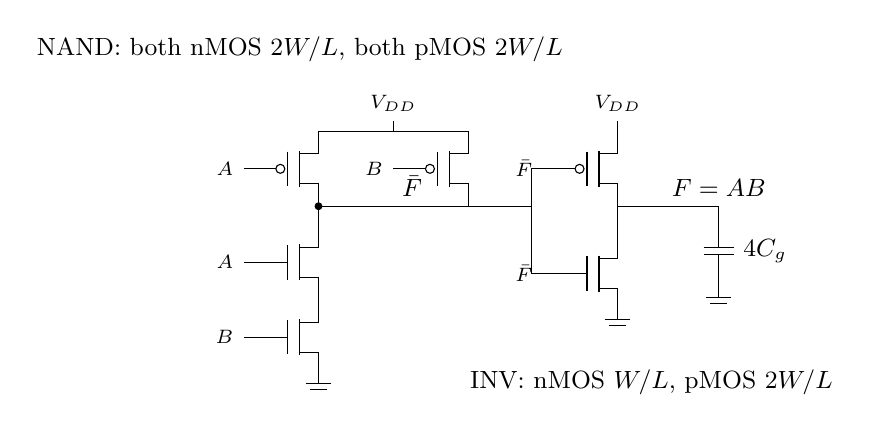
\begin{tikzpicture}[scale=.95,font=\small]
\mos{0}{3}{A}{1}\mos{2}{3}{B}{1}\draw(.25,3.5)--(2.25,3.5);\rail{1.25}{3.5}{V_{DD}}
\draw(.25,2.5)--(2.25,2.5);\draw(.25,2.5)--(.25,2.25);\mos{0}{1.75}{A}{0}\mos{0}{.75}{B}{0}\ground{.25}{.25}
\draw(.25,2.5)--(3.1,2.5);\draw(3.1,1.6)--(3.1,3)--(3.25,3);\draw(3.1,1.6)--(3.25,1.6);\fill(.25,2.5)circle(1.5pt);\node[above]at(1.5,2.5){$\bar F$};
\mos{4}{3}{\bar F}{1}\mos{4}{1.6}{\bar F}{0}\rail{4.25}{3.5}{V_{DD}}\ground{4.25}{1.1}\draw(4.25,2.1)--(4.25,2.5)--(5.6,2.5)node[above]{$F=AB$};
\draw(5.6,2.5)--(5.6,1.95);\draw(5.4,1.95)--(5.8,1.95);\draw(5.4,1.85)--(5.8,1.85);\ground{5.6}{1.4}\draw(5.6,1.85)--(5.6,1.4);\node[right]at(5.8,1.9){$4C_g$};
\node[above]at(0,4.3){NAND: both nMOS $2W/L$, both pMOS $2W/L$};
\node[below]at(4.7,.45){INV: nMOS $W/L$, pMOS $2W/L$};
\end{tikzpicture}\end{center}
\newpage\section*{7. Static complementary CMOS (15 points)}
Each full-expression bar is preserved from the printed prompt; there are no inner complemented input variables. The supplied handwritten networks have the correct series/parallel connectivity and are retained. All nMOS bodies are tied to VSS and all pMOS bodies to VDD. Each PDN realizes the expression under the bar; its dual PUN realizes the complement.

\subsection*{(a) $F=\overline{X(Y+Z)}$ -- 6 transistors}
PDN: X in series with Y parallel Z. PUN: X parallel the series pair Y,Z.
\begin{center}\begin{tikzpicture}[scale=.82,font=\small]\mos{0}{4}{Y}{1}\mos{0}{3}{Z}{1}\mos{2.5}{3.5}{X}{1}
\draw(.25,4.5)--(2.75,4.5)--(2.75,4);\draw(.25,2.5)--(.25,2.2)--(2.75,2.2)--(2.75,3);\rail{1.5}{4.5}{V_{DD}}
\mos{1.2}{1.7}{X}{0}\mos{0}{.7}{Y}{0}\mos{2.5}{.7}{Z}{0}
\draw(.25,1.2)--(2.75,1.2);\draw(.25,.2)--(2.75,.2);\ground{1.5}{.2}
\draw(1.45,2.2)--(4,2.2)node[right]{$F=\overline{X(Y+Z)}$};\fill(1.45,2.2)circle(1.5pt);\end{tikzpicture}\end{center}
\subsection*{(b) $F=\overline{XY+Z}$ -- 6 transistors}
PDN: the series pair X,Y in parallel with Z. PUN: Z in series with X parallel Y.
\begin{center}\begin{tikzpicture}[scale=.82,font=\small]\mos{1.2}{4}{Z}{1}\mos{0}{3}{X}{1}\mos{2.5}{3}{Y}{1}
\draw(.25,3.5)--(2.75,3.5);\rail{1.45}{4.5}{V_{DD}}\draw(.25,2.5)--(2.75,2.5);
\mos{0}{2}{X}{0}\mos{0}{1}{Y}{0}\mos{2.5}{1.5}{Z}{0}
\draw(2.75,2)--(2.75,2.5);\draw(.25,.5)--(2.75,.5)--(2.75,1);\ground{1.5}{.5}
\draw(.25,2.5)--(4,2.5)node[right]{$F=\overline{XY+Z}$};\fill(.25,2.5)circle(1.5pt);\end{tikzpicture}\end{center}
\newpage\subsection*{(c) $F=\overline{X+Y(W+Z)}$ -- 8 transistors}
PDN: X in parallel with Y in series with W parallel Z. PUN: X in series with Y parallel the series pair W,Z.
\begin{center}\begin{tikzpicture}[scale=.82,font=\small]\mos{0}{5}{W}{1}\mos{0}{4}{Z}{1}\mos{2.5}{4.5}{Y}{1}\mos{1.2}{3}{X}{1}
\draw(.25,5.5)--(2.75,5.5)--(2.75,5);\rail{1.5}{5.5}{V_{DD}}\draw(.25,3.5)--(2.75,3.5)--(2.75,4);
\mos{0}{1.5}{X}{0}\mos{2.5}{2}{Y}{0}\mos{2}{1}{W}{0}\mos{4}{1}{Z}{0}
\draw(1.45,2.5)--(.25,2.5)--(.25,2);\draw(.25,2.5)--(2.75,2.5);\draw(2.25,1.5)--(4.25,1.5);
\draw(.25,1)--(.25,.5)--(4.25,.5);\ground{2.25}{.5}
\draw(1.45,2.5)--(5.2,2.5)node[right]{$F=\overline{X+Y(W+Z)}$};\fill(1.45,2.5)circle(1.5pt);\end{tikzpicture}\end{center}
The executable evaluates all 8, 8 and 16 input words using switch-graph connectivity. Exactly one of VDD or VSS is connected to F in every case, and its voltage polarity matches the original Boolean expression. All 32 checks pass; these are ideal connectivity checks, not a fabricated analog/PVT characterization.

\section*{Source reconciliation and reproduction}
The student's correct Q2 constants, quadratic passive-delay explanation, Q4 nominal threshold/interior regions, Q5 strength comparison, and Q7 diagrams are retained. Q1 short answers are expanded where steps or physical conditions were omitted. Q3's graded $20C_g$ convention is explicitly conditional. Q6's capacitance mistake is corrected by strengthening the NAND nMOS devices, yielding $7RC_g$.

Run \texttt{python verify\_q2\_q7.py} and \texttt{python verify\_q3\_q6.py} in this folder. They regenerate the analytical CSV/JSON evidence. No process model is needed. Both this report and \texttt{exam.tex} are standalone pdfLaTeX documents; all circuits are native TikZ vectors, with no scan-image dependency. See \texttt{SOURCES.md}, \texttt{sources.json} and the original two-page extraction for provenance and limitations.

\section*{Primary technical references for Q1}
\begin{enumerate}[leftmargin=7mm,itemsep=5pt]
\item Synopsys, \href{https://www.synopsys.com/articles/finfet-design.html}{FinFET Design Insights and Reliability}: fin geometry, effective electrical width and quantized sizing. The general device facts are used, not its historical process-roadmap predictions.
\item Intel, \href{https://www.intel.com/content/www/us/en/newsroom/news/powervia-test-shows-industry-leading-performance.html}{PowerVia Test Shows Industry-Leading Performance}, 2023: backside routing separates power from signal wiring and improves voltage droop. Product-release forecasts are not part of the answer.
\item TSMC, \href{https://www.tsmc.com/english/dedicatedFoundry/technology/cowos}{CoWoS technology}: silicon-interposer die integration; detailed manufacturing order is technology dependent.
\item TSMC, \href{https://patents.google.com/patent/US11094671B2/en}{US11094671B2, Package with thinned substrate}, Figure 11: a disclosed example of die-to-interposer-wafer bonding, encapsulation, backside processing and later substrate assembly. This supports a representative sequence, not a universal commercial recipe.
\end{enumerate}
\end{document}
